% TRANSLATION UNIT: translate this file only.
% ===========================================================================
%  01 — Planteamiento del problema
%  The \section title is the canonical (Spanish) chapter name; the body prose
%  is written in ENGLISH and translated to Spanish later.
% ===========================================================================

\section{Planteamiento del problema}

% DONE: Problem statement written in English. The problem is stated as a
% measured condition (Banco de la República, February 2024: 16.4 % answer the
% Big Three), then narrowed to what a software project can address and what it
% does not claim, the research question is stated once, and the architecture
% is justified from the shape of the problem rather than from fashion. The
% causes-and-effects tree is Figure~\ref{fig:arbol-causas-efectos}. No \todo
% remains; no claim exceeds the evidence inventoried below.

% ---------------------------------------------------------------------------
% CLAIMS INVENTORY — every prose claim is listed here with its evidence.
% The prose below makes only these claims.
% ---------------------------------------------------------------------------
% EVIDENCE: 16.4 % of Colombians answer the Big Three (compound interest,
%   inflation, risk diversification) correctly → banrep2024financial abstract,
%   read on the banrep.gov.co record page; the full PDF is served through a
%   script-only button with no file URL (fuentes-acceso.md:85). Date 2024-02-29
%   and the "high inflation environment" framing are the publication record.
% EVIDENCE: the five causes and five effects of the tree are the author's own
%   synthesis, laid out in the proposal → docs/anteproyecto/situacion-problema.md,
%   docs/anteproyecto/justificacion.md and the figure source
%   docs/informe/figures/fig-arbol-causas-efectos.dot.
% EVIDENCE: what the platform does not claim (no causal effect on the 16.4 %,
%   no controlled learning-outcome experiment, no behavioral change) and what
%   it does claim (teach, practice, maintain, in Spanish and Colombian context)
%   → docs/anteproyecto/alcance.md and the evaluation being of an artifact, not
%   a pedagogical trial (docs/informe/04-instrumentos-validacion.md).
% EVIDENCE: content changes on a different cadence than the code that serves
%   it; FR-007/FR-008/FR-013 require drafting, review, publication and
%   versioning → specs/001-fintcart-platform/spec.md:136-152.
% EVIDENCE: money and rates must never be floats; FR-028 is the non-negotiable
%   arbitrary-precision requirement and FR-019/FR-021 bind the calculators to
%   it → specs/001-fintcart-platform/spec.md:177-191 (FR-019/FR-021), :191 (FR-028).
% EVIDENCE: the parts evolve independently because each domain is a separate
%   service with its own database; cross-service consistency only via saga →
%   .specify/memory/constitution.md:76,89,120,136 (restated as requirements in
%   chapter 06).

% ---------------------------------------------------------------------------
% BODY
% ---------------------------------------------------------------------------

Financial literacy is a measurable deficit, not a diffuse worry. The most
widely used instrument asks three questions --- about compound interest,
inflation, and risk diversification --- and a person is counted as financially
literate only if all three are answered correctly. In Colombia, the most
recent national measurement by the Banco de la República, published in
February 2024 and explicitly framed in a high-inflation environment, reports
that 16.4 \% of the population clears that bar \parencite{banrep2024financial}.
The figure and its date are read from the publication's public record page;
the full PDF is served only through a script-driven button with no direct file
URL, so this chapter uses the reported measurement and builds no argument on
the body of the report. Read plainly, the number says that fewer than one
Colombian in six can correctly handle the three operations on which almost
every ordinary financial decision rests: the compounding of interest, the
erosion of purchasing power, and the diversification of risk. The shortfall is
not a matter of temperament or of taste; it is a measurement of what a
population can and cannot do with money, and it is the condition this project
responds to. It also matters that the measurement exists at all: a problem
that is counted can be addressed deliberately, and the count turns a broad
intuition --- that many people handle money poorly --- into a specific,
checkable fact about a population.

Behind that number stand causes and effects worth drawing before they are
discussed, because the drawing keeps the argument honest about what is cause,
what is problem, and what is consequence. Figure~\ref{fig:arbol-causas-efectos}
arranges them as a tree: five causes on the left, five effects on the right,
and the measured condition at the center. The causes are that financial
concepts are never taught in the first place (inflation, rates, interest);
that teaching stays theoretical, without practice or simulation; that habits
are formed by imitation rather than by decision; that the tools available are
in English or foreign to the Colombian context; and that content is updated
only on paper. Each cause names a lever that a digital platform can in
principle pull: it can teach the concepts, make practice immediate, offer a
place to rehearse decisions, speak the user's language and currency, and keep
its material current. The tree is the proposal's own diagnosis drawn in one
place, and it is reproduced here because the document that follows aims at the
left side of the tree --- the causes --- rather than at the right side, which
no software alone can undo. The effects are the mirror of those causes in people's
lives: decisions about credit and saving that impoverish rather than build;
real income eroded by an inflation that is not understood; the absence of
planning for retirement and risk; a widening gap between those who master
finance and those who do not; and dependence on third parties for everyday
economic decisions. At the center sits the problem itself: low financial
literacy in the Colombian population, 16.4 \% with basic knowledge.

\begin{figure}[htbp]
  \centering
  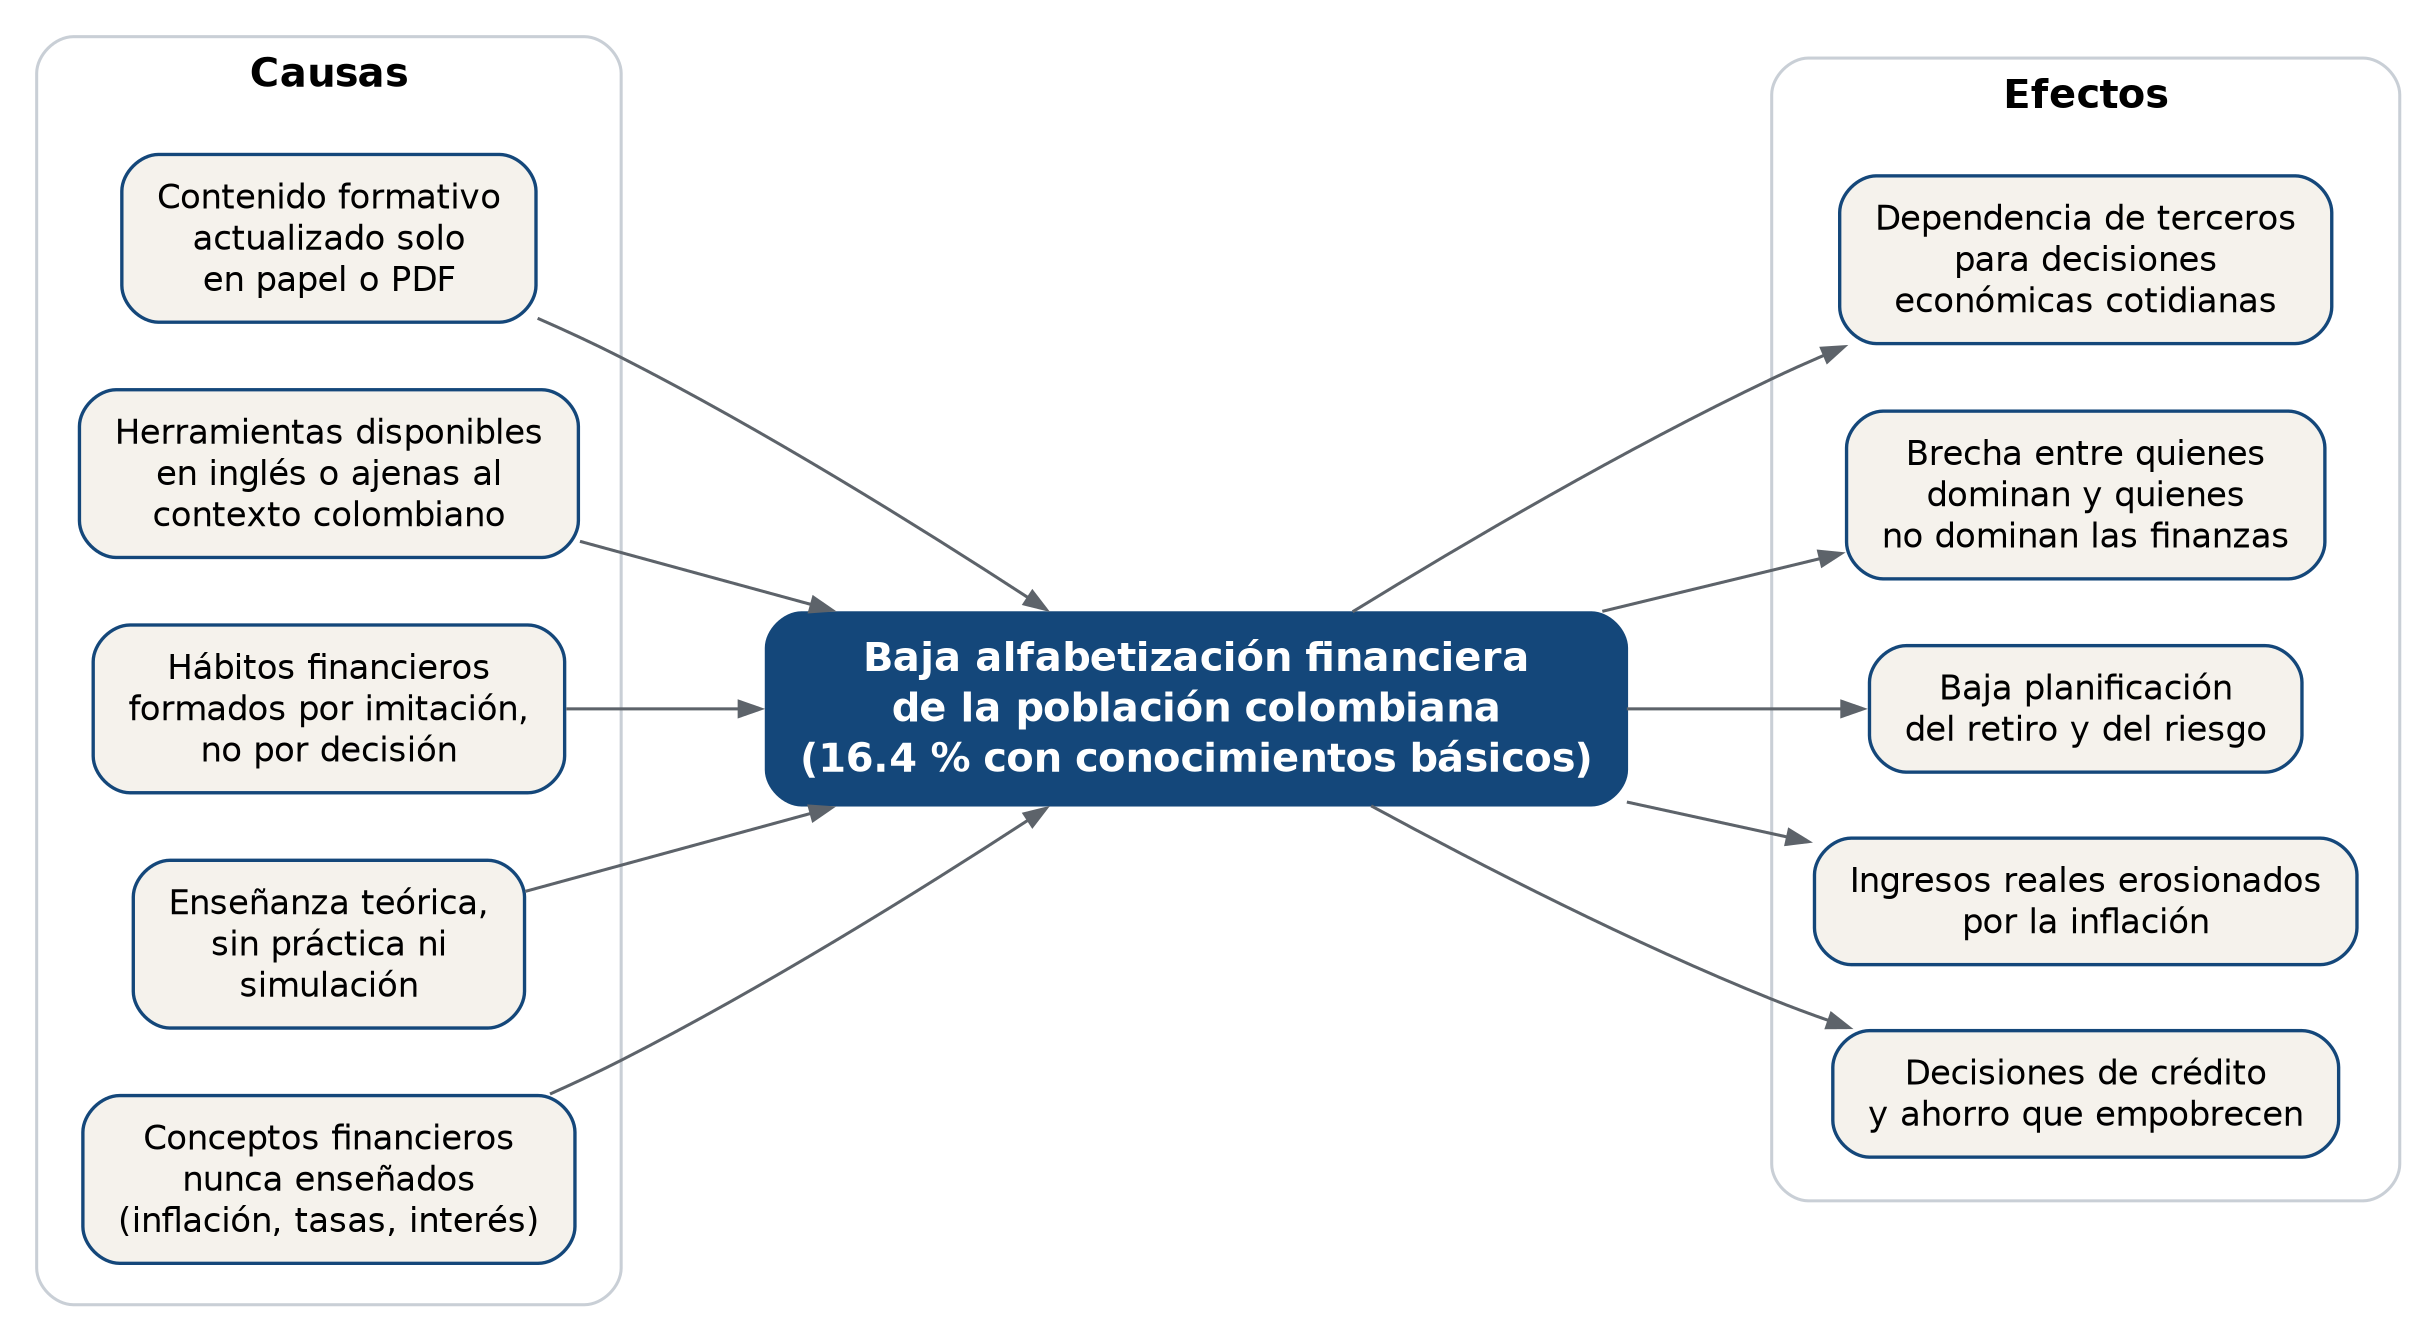
\includegraphics[width=\textwidth]{fig-arbol-causas-efectos.png}
  \caption{Causes and effects tree of the problem.}
  \label{fig:arbol-causas-efectos}
\end{figure}

The tree is the whole problem, and it is larger than any single artifact.
Financial literacy is a long-run social outcome shaped by schooling,
households, regulation, and access to formal finance; no platform, however
well built, can raise the 16.4 \% by itself, and this project does not claim
that it will. Three refusals delimit the claim. The project does not claim to
raise Colombia's measured literacy, because that would require an evaluation
of learning outcomes in a controlled population, which this thesis does not
perform. It does not claim to change financial behavior, a claim that would
demand behavioral data the project neither collects nor evaluates. And it does
not claim to replace financial advice or to decide on its students' behalf:
the calculators compute, and the decision remains the student's. What the
project does claim is narrower and, for that reason, defensible. It builds the
instrument through which accurate, contextualized, interactive financial
education can be delivered and kept current in the Colombian context.
Concretely, the platform undertakes four things and no more: it teaches
financial concepts through readable, reviewed articles; it lets a student
practice what those articles explain, by running calculators over realistic
figures in Colombian pesos; it keeps that material current through a
publishing flow in which an editor writes and an editorial coordinator
approves; and it does all of this in Spanish and in the Colombian monetary
context, so that neither language nor currency stands between the student and
the concept. The slice of the problem that software can actually address is
the availability and maintainability of good material --- the causes on the
left of the tree, which concern content, practice, language, and freshness ---
not the social outcome on the right.

From that narrowing the research question follows, and it is stated here once,
in full: how to build a financial-education platform on a microservices
architecture that supports learning, practice, and content maintenance in the
Colombian context. The architecture is named in the question on purpose: it is
not a postscript to the problem but part of its shape, because the three
undertakings just listed --- teaching, exact practice, and maintained
content --- pull a single system in three different directions, and the
question asks how a structure can hold them together without any one of them
degrading the others. The rest of this document answers the question with an
artifact, not with an experiment. The answer is an implemented platform, built
against a written specification and measured with unit, integration, and
end-to-end tests; Chapter 5 records the method, Chapter 6 the requirements,
Chapters 7 and 8 the architecture and the data model, Chapter 10 the
implementation, and Chapters 11 through 13 the verification and the measured
results. What the document deliberately does not contain is a trial of
learning outcomes. Whether the platform moves the 16.4 \% is a question the
artifact makes answerable, not a question this thesis answers. By artifact is
meant the platform itself --- its sources, specifications, migrations, and
tests --- all of which exist and can be inspected in the repository that
accompanies this document.

The architecture follows from the same narrowing, and it is chosen because the
problem has three structural features that a single, undivided application
serves badly. They are not three justifications in search of a technology;
they are three constraints that any honest solution to the problem must
respect, and they map one to one onto the requirements of Chapter 6.

First, content changes on a different cadence than the code that serves it. An
article is not software: it is drafted, revised, and retired on the schedule
of a curriculum, while the code that renders it changes on the schedule of an
engineering team. Articles are drafted, reviewed, published, and revised, and
every revision must leave a trace of who wrote it and who approved it; the
requirements that encode this --- curation by an editor and an editorial
coordinator, versioning, and a publication flow --- are \code{FR-007},
\code{FR-008}, and \code{FR-013} in Chapter 6. Content coupled to its
deployment cannot accept a correction without redeploying the whole system, so
the problem demands that content be data with its own life cycle, served by a
service that can be replaced without touching the rest. This is the first
reason the platform is not a single undivided application.

Second, some of what the platform computes must be exact, and exactness is the
one property a general-purpose runtime will give away for free if no one stops
it. Money and interest rates are not quantities that may be rounded through
binary floating point: a rounding error in a savings projection is a wrong
answer dressed as a right one, and in a platform whose whole purpose is to
teach, a subtly wrong answer is worse than no answer. The requirement that
fixes this, \code{FR-028}, is non-negotiable, and the calculators a student
runs (\code{FR-019}, \code{FR-021}) inherit it. That is a computational
demand, not a stylistic one, and it earns its own service: the simulator
service, where formulas are parsed and evaluated, must be built so that
exactness cannot be silently traded away. A service that must be exact is a
service that must be isolated from the parts that merely have to be fast.

Third, the parts evolve independently because they are different domains with
different owners and different failure modes. The catalogue of articles, the
evaluation of formulas, the identity of students, and the delivery of
notifications change for different reasons and at different speeds, and a
failure in one --- an unavailable mail server, say --- should not be able to
take down the reading of an article. Keeping them as separate services, each
with its own database, is what lets one part be corrected without dragging the
others along, and it is what the repository's constitution encodes as
non-negotiable --- database-per-service, no cross-service access, and
consistency only through the saga pattern, restated as requirements in
Chapter 6. The same separation is what makes the system maintainable in the
long run, which is the very property the fifth cause of the tree --- content
that ages --- demands.

None of these three pressures is about fashion. Microservices are not adopted
here because they are contemporary or because the industry happens to speak of
them; they are adopted because a problem whose content, computation, and
domains each demand a different discipline is precisely the problem a set of
independently deployable services exists to solve. The chapters that follow
turn this problem statement into that system, and the reader will meet each of
the three pressures again as a concrete requirement in Chapter 6 and as a
concrete service in Chapter 7.
